% In this section:
% This should contain all of the decisions regarding the design. If the reader has a question (`why did they do/choose that?' then this is where they look)

% Things to include here:
% Choosing motors
% Choosing gears/etc
% Choosing servos

\chapter{Design Outline}\label{design outline}\label{section \thechapter}\todo{Is this the best name for this chapter?}

\mySection{Aims and motivations}{\AH}\label{outline: aims and motivations}
    \towrite{aims and motivations}


\section{Robot body and movement}\label{outline: body and movement}

    \mySubsection{Chassis and materials}{\AK}
        An important consideration when deciding on a material for the body and base of the robot is the penetration into the sand. A denser material will cause the robot to sink more, but lighter materials will mean a compromise in strength, stability, or price. However, if the wheels or tracks of the robot are wise enough, there may be some freedom when deciding what materials the components of the robot should be made of.\\
        Researchers at the Georgia Institute of Technology have been able to vary the strength of the supporting ground by using varying air flow from beneath.\cite{Qian} This has allowed them to vary the stiffness of the sand and observe the performance of a robot on these surfaces.

        The robot should be made to be water resistant; contact with water at some point is inevitable and water coming into contact with the electrics would reduce the lifespan and reliability of the machine. Damage caused by sand should also be a consideration: the machine is likely to come into contact with a substantial amount of sand. Sand is silica, which is very abrasive; if this abrasion occurs around the more sensitive areas of the machine it could cause extensive damage. Sandusa is a range of beach products that are water- and sand-proof.\cite{sandusa} This is due to a smooth nylon material that allows sand to slide off easily combined with an inner waterproof lining. This material could be used to protect the robot.
        \towrite{materials and chassis}


    \mySubsection{Movement}{\SW}
        In considering a robot's locomotion, the terrain over which it will travel (sand -- potentially damp) and its purpose (drawing) are center-stage. The robot must have sufficient traction to travel over a beach. When considering the requirement that it draw, it must be able to turn as tightly as instructed to avoid incongruity between programmed and drawn images. It may also be possible to incorporate any turning limitations into the child's programming interface, such that an impossible turn cannot be instructed. It would also be far from ideal for the robot to obscure any lines it had already drawn when pathing back over them.

        The main methods of robot locomotion that might be relevant are wheeled (or caterpillar tracked), walking, rolling, or slithering. Considering the scope of this project, and the budget available, the latter options are not viable. Companies such as Boston Dynamics have budgets of millions of dollars to work on the development of walking technology -- achieving a robot capable of walking is a significant feat, even before considering drawing. While rolling or slithering may potentially be workable, they would contribute significant design complications to any kind of `on/off' functionality. Flying private drones have increased in popularity dramatically; in considering a drone type robot as an option, the main challenges are the extreme comparative difficulty of achieving flight compared with traction and drawing a line in the sand. Creating a flying drone from scratch would pose many challenges, which it is unlikely we could surmount with this project's resources. The marker design also poses significant challenges -- a marker fixed rigidly to a drone is likely to interfere with flight and a free-hanging marker runs the risk of not providing enough pressure to create a line. The most viable locomotion solutions are caterpillar tracks and wheels.\\
        Caterpillar tracks combine very capable terrain handling with on-a-point turning, however they are very likely to disrupt the line left behind the robot, especially when on-a-point turning.  With the right design and material, wheels might prove sufficiently able to handle the terrain and also cause limited harm to the robot's drawn lines. Such wheels would need to have a large surface area and be made of a reasonably soft material (\eg soft touch plastic) -- minimizing the robot's overall weight would also be important in making such a design choice viable. Although wheels open opportunities in terrain handling and line preservation, they come up short of caterpillar tracks on turning ability. A short wheelbase might go some way to improve this. There is also the potential of a three-wheel configuration, instead of four (or more) wheels -- this was implemented in Disney's BeachBot (Section~\ref{sand-drawing robots}) to the benefit of the robot’s turning circle. It should be noted that a three-wheel design raises stability concerns. Ultimately the decision between caterpillar tracks and wheels comes to a question of whether, or to what extent, the child instructing the robot should be limited in their design.
        \towrite{movement: the decision}


    \mySubsection{Digging mechanisms}{\SW}\label{outline:drawing tool}
        At its most basic level, a beach-scale sand drawing robot need only leave a line in the sand wherever it travels, in order to produce a picture -- this poses a severe constraint on what can be drawn. In the case of our educational robot, the child would have the limitation of instructing the robot to draw a picture with only a single continuous movement. This `always on' approach to the drawing mechanism can be improved upon.

        Instead of fixing the robot's marking implement, it could be built to raise or lower, adding `on/off' drawing functionality. The marking implement, or `marker', could be fitted to an actuator to achieve this. The actuator could be linear or rotary; a linear actuator would lend itself to a marker below the robot chassis, while a rotary actuator would be more appropriate for a marker behind the chassis, like a rake tooth (as is being used in Figure~\ref{fig: andres amador}). A rear mounted, rake-like design might provide a more fluid, pulling movement through the sand. There are precedents for this positioning choice: Disney's BeachBot (Section~\ref{sand-drawing robots}) and plough attachments for tractors. While the addition of an actuator significantly improves the robot's drawing flexibility, it would be vulnerable to sand in its mechanism and would add cost, should one not be salvageable from spare parts. The use of an actuator would also place a small requirement on the robot's power supply.\\
        The marker itself needs to exert sufficient force on the sand to leave a line behind the robot, without acting as a brake -- this would inhibit the robot's movement. Inhibition of the robot's movement would lead to significant deviation in the drawn image compared to the programmed image. The key to avoiding this is to create a marker with appropriate depth; the marker should not penetrate so deep in the sand as to invite significant resistance to its motion, while reaching deep enough to leave a sufficient (\emph{i.e.} visible) line.\\
        Implementing software to vary the depth of the marker could serve to mitigate any issues arising from resistance, and also could ensure trouble does not arise on uneven beach area. The limitations here lie within the realm of software development, and potentially the requirement that the actuator provide feedback.\\
        Within these parameters the marker itself could be varied -- for instance having multiple markers would provide a different pattern to the line. These multiple markers could be fitted to more actuators (with the potential of substantially increased cost) to allow for a variable line width.

        An alternative marker approach would be that of a cylindrical `drum'. Such a cylinder could have a pattern embossed upon it that would leave a pattern as the robot's marking. Gunilla Klingberg's `sand machine' (Section~\ref{art review}, Figure~\ref{fig: sand machine}) uses this approach. This approach could be implemented with `on/off' functionality, but would allow for only a preset pattern in the line. The implementation of a patterned line of varying width (\eg multiple drums with raising and lowering ability) could prove very problematic. Such an implementation of this method would be best achieved in a manner similar to NASA's RASSOR digging robot -- a drum separate from the locomotion mechanism that can be lowered and raised.\cite{Siceloff2013} In a similar way, the NASA's Curiosity rover leaves the pattern for ``JPL'' in Morse code in its tracks as it travels across the Martian surface.

\section{Electronics and control}\label{outline: electronics and control}
    \mySubsection{Guidance methods}{\CL \SW}\label{outline:guidance}
        In order to draw an image in a given area, the robot will need to be guided by some system. \towrite{Guidance: manual controls}

        The robot could also be autonomous. Three options for autonomous guidance have been explored: ultrasound, lasers, and \gls{GPS}. There are many other guidance systems that have not been mentioned such as tethering, grid systems, infrared, and more. These other guidance systems have not been mentioned because they are either too complex, have too small of a range, or it is not possible to make an autonomous robot using the particular guidance system.

        \paragraph{Ultrasound} detection systems comprise two parts, a transmitter and a receiver. The transmitter emits a sound at a defined frequency (typically around \SI{40}{\kilo\hertz}) and the receiver collects the sound reflected back by the obstacles. The distance to the objects is calculated by measuring the time taken by the sound to return to the receiver.\\
        Ultrasound is normally used to measure distances because sensors because they are cheap and very simple to use. Ultrasound has a range of \SIrange{1}{250}{\centi\meter} and an effective working angle of approximately 30\dg.\cite{ultrasoundrobots} The working angle of ultrasound can be pictured as a cone that has an angle of 30\dg, where measurements of distance will be more accurate within the centre of the cone and less accurate towards the sides. Other things to be considered with ultrasound are the shape of the obstacle and the inability of ultrasound to make measurements of distance when the sensor is very close to an obstacle. This is due to the sensor needing a large enough return time for the wave that is reflected; if the a sensor with a long transmitting wave duration is used, it may not be able to detect an object in close proximity since the wave will return too quickly, before the sensor can started receiving.\\
        Ultrasound is normally used to measure distances because sensors because they are cheap and very simple to use. Ultrasound has a range of \SIrange{1}{250}{\centi\meter} and an effective working angle of approximately 30\dg.\cite{ultrasoundrobots} The working angle of ultrasound can be pictured as a cone that has an angle of 30\dg, where measurements of distance will be more accurate within the centre of the cone and less accurate towards the sides. Other things to be considered with ultrasound are the shape of the obstacle and the inability of ultrasound to make measurements of distance when the sensor is very close to an obstacle. This is due to the sensor needing a large enough return time for the wave that is reflected.\todo{how would US be used to guide the robot to draw an image?}

        \paragraph{Lasers} could be used in different ways to guide the robot. One way is to have a guidance system for freely chosen courses, which uses a laser beam that hits strategically placed mirrors to reflect the beam. The on-board controller then analyses the angles that the beam is reflected at and uses triangulation to determine the position of the robot. Another method is to use a laser range finder that emits a beam and measures the time taken to reflect off the object and return to the sender. Both methods are accurate to within a few millimetres but the first method is the more accurate of the two.\\
        Laser guidance systems can be used in any environment and have a range of several metres. They have a range of several metres and out of the three guidance systems mentioned are the most accurate. The markers for the laser beams have to be set every \SIrange{2.5}{4.5}{\meter} and should not be blocked. The robot must be able to see multiple markers (mirrors) at once so that it can determine its precise location. The only disadvantages of using a laser guidance system are that they are the most complicated and the most expensive of the three systems discussed.\todo{mention LIDAR?}

        \paragraph{\gls{GPS}} receivers use a constellation of 31 satellites orbiting over 20,000 km, with a revolution period of 12 hours (as of February 1st 2016). Every satellite transmits data packs, which contains: the time, current position, other satellites positions and other information. The \gls{GPS} receiver receives the information about position from the radio transmissions of the satellites it can track. 4 satellites are normally used to compute the position. Although it is possible to measure the position with fewer satellites, the margin of error is large.\\
        \gls{GPS} \glspl{shield} are inexpensive and as a guidance system, obviously have a very large range.  However, the accuracy of \gls{GPS}, which may be within few metres, may depend a number of things such as signal noise, satellite position, and obstruction from tall buildings. Therefore, if GPS is to be used as the guidance system for the robot, then its worth considering a location that is isolated from tall building when it comes to the testing of the robot because signal noise can cause errors up to \SI{10}{\meter} and obstruction from tall buildings can cause errors three times more than the error from signal noise.\cite{gpsbasics} There are ways of getting the accuracy of the \gls{GPS} down to a few centimetres by using correction methods such as a differential \gls{GPS}, using a combination of \gls{GPS} and some other local positioning systems such as electronic compasses or \gls{INS}. However, these correction methods are complex and expensive and therefore they are not feasible solutions to increasing the accuracy of \gls{GPS}.
        % Luke, 07/03: INS-corrected GPS is not complex or expensive, and is entirely feasible.

        \towrite{electronics: kill switch}


    \mySubsection{Control platform}{\SSB}\label{outline: control}
        \begin{figure}%{I}{0.45\textwidth}
            % \vspace{-11pt}
            \centering
            \begin{subfigure}[b]{0.45\textwidth}
                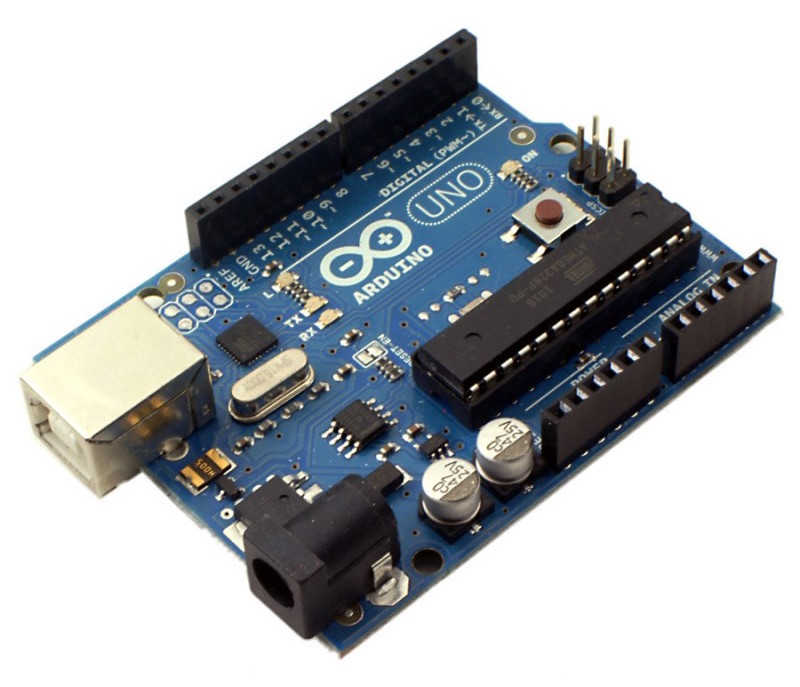
\includegraphics[width=\textwidth]{Files/arduino}
                \caption{An Arduino UNO.}
                \label{fig: arduino}
            \end{subfigure}
            ~
            \begin{subfigure}[b]{0.45\textwidth}
                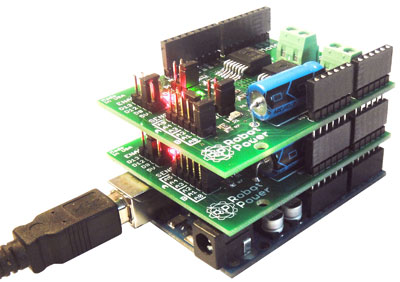
\includegraphics[width=\textwidth]{Files/arduino_with_shields}
                \caption{An Arduino with 2 \glspl{shield} attached.}
                \label{fig: arduino shields}
            \end{subfigure}
            \caption{\small (Retrieved from \citen{robotshop} on 2016--01--25)}
            \label{fig: arduino and shields}
            % \vspace{-20pt}
        \end{figure}
        The robot will need a control system to plan and control its movement, and to control the drawing tool. This system could be developed from proprietary systems or built by the group for this specific application.

        \paragraph{\gls{Arduino}} (Figure~\ref{fig: arduino}) is an open-source micro-controller system designed for embedded systems control. It can be expanded by the use of \emph{\glspl{shield}} (Figure~\ref{fig: arduino shields}), circuit boards designed to attach to header pins on the primary micro-controller board to created stacks of circuits with different functions. This would allow us to build a control system for the robot using pre-designed circuits. \Glspl{shield}, which can be bought from many electronics suppliers, are available to add bluetooth, GPS, motor control, and many other functions to the primary circuit.\\
        There is a large online community supporting the \gls{Arduino} project, which could be leveraged to solve programming difficulties if they arise. The \gls{Arduino} project provides an integrated development environment (IDE); the \gls{Arduino} is programmed using a language based on the C and C++ languages.
        \paragraph{Netduino} is a variant of the \gls{Arduino} which runs on Microsoft's .NET framework. The online support community for this system is smaller, although some group members (\AG, \LY) have a pre-existing familiarity with the .NET framework.\\

        \todo[inline]{electronics: rework the following paragraphs}
        \paragraph{Raspberry Pi} is a small single-board computer developed in the UK to promote access to computer science education in schools. Because on this, the platform is already widely used in an educational setting and thus would allow this project to be more easily integrated into the teaching of computer science. The computer itself is low-cost (<\pounds{50}\todo{check the price of Raspberry Pi}).\\
        The Raspberry Pi Foundation also produce smaller versions of the Raspberry Pi computer which are designed for use in embedded systems. These boards are less customizable than the Arduino system. However, it is compatible with the Python language, which has an extensive support community online and is familiar to all the group, as well as C, C++, Java, and others.

        \paragraph{A micro-controller} integrated circuit could be used in a purpose-built system to control the robot. This would require the design of all the supporting electronics. The microprocessor would need to be programmed in a low-level assembly language or a language designed specifically for the micro-controller product we use.\\
        These components would be cheaper than commercially available systems, but would require much more electronics design work and fabrication.


    \mySubsection{Control theory}{\LY}\label{outline: control theory}
        Control theory lies at the interface between positioning systems and control platforms.
        Given some target movement pattern, control theory concerns the way we interpret positioning data and use this information to generate commands for the robot.

        Our primary concern on this front is noise.
        Each positioning system carries a distinct class of noise associated with the positioning information it provides---for instance,
        \begin{itemize}
            \item GPS carries noise in absolute position,
            \item a compass carries noise in absolute angular position,
            \item an accelerometer carries noise in relative position, and
            \item a gyroscope carries noise in relative angular position.
        \end{itemize}
        Each positioning system may also have other deficiencies, including a low rate of update, as is found in GPS and electronic compasses.
        Fortunately, the Kalman filter provides a powerful and well-understood method for utilizing multiple sources of positioning data, in order to collectively overcome each of their individual deficiencies.

        Since implementing the Kalman filter would place substantial strain on our financial and technical capabilities, we explored an alternative method for coping with noise.
        Instead of dealing with noise at the control level, we sought to deal with it at the specification level---that is, by restricting our target movement patterns to those that are robust to noise.

        In the following, we describe our findings with regard to this alternative method and explain how the Kalman filter can be applied to this project.

        \subsubsection{Noise-robust paths}
        Inspired by emergent phenomena in many-body systems, we consider the existence of movement patterns whose emergent art is robust to noise.
        Just as thermal agitation does not preclude mechanical transport, it may be that noisy positioning data does not preclude large scale order in the form of art.

        For simplicity, we consider movement patterns characterised by continuous paths in the plane.
        In this context, we seek a class of paths for which noise is washed away at sufficiently coarse-grained representations.
        This coarse-graining is naturally provided by viewing the paths at further distances with fixed resolution.
        We work in the absence of explicit error correction to ease our technical burden, and in the absence of GPS to minimise our reliance on external conditions.
        Explicit error correction will be taken up in the next section on noise-robust control.

        By analogy with many-body systems, we expect that the emergent large scale order of noise-robust paths should be scale-invariant.
        One such class of paths is the fractal path\footnote{Commonly referred to as fractal \emph{curves} in the mathematical literature.}.
        They exhibit scale-invariance by way of self-similarity, in addition to being straightforward to generate at scale.
        Indeed, our simulations suggest that some families of fractal paths can generate large scale order despite accumulating small scale noise.

        Given any target path, our computer simulation mimics the robot's movement as follows.
        It discretises the path into a sequence of straight line segments, each of which is stored as a 2-dimensional vector and extends no more than some fixed length $r_0$.
        Since $r_0$ acts as the maximal length of an elementary line segment, it must be chosen to be small compared to all other length scales of the system---namely, the size of the intended drawing.
        Each vector in the sequence is then transformed to its noisy counterpart by replacing its radial and angular components with normally distributed random variables with mean equal to the original value and standard deviation given by the standard error inherent to our system.
        The resulting path, generated by traversing each noisy vector in sequence, is one sample of the random process.
        Since our goal is to generate visual art for the eye, the resulting paths are evaluated by comparing them to their target paths by eye.

        \begin{listing}[pbt]
            \inputminted{mathematica}{Code/gestalt.m}
            \caption{Mathematica code used to sample noisy paths through four test images. A target path is generated for each high-resolution colour image by converting it to a 100-by-100 pixel black-and-white image, and applying Mathematica's optimisation algorithm for finding the shortest tour along the black pixels. Three noisy paths are sampled for each target path.}
            \label{lst:gestalt}
        \end{listing}

        \begin{listing}[pbt]
            \inputminted{mathematica}{Code/koch.m}
            \caption{Mathematica code used to sample noisy paths through Koch curves of various length. The target path is generated by utilising the mapping from the Thue-Morse sequence to directions that converge to the Koch curve. Four noisy paths are sampled for each target path.}
            \label{lst:koch}
        \end{listing}

        This procedure is implemented in Listings~\ref{lst:gestalt} and \ref{lst:koch}.
        With positioning data from an electronic compass and a linear accelerometer, we estimate that noise in the robot's movement introduces an angular standard error of 1 degree~\cite{honeywell} and, to be safe, a radial standard error of at most a tenth of each discrete segment.
        These are implemented as \mintinline{mathematica}{et = 2*Pi/360} and \mintinline{mathematica}{er = 0.1} in the listings, where we have used $r_0 = 1$.
        Note that the absolute angular positioning data from the compass is utilised in a sub-optimal manner---instead, an absolute coordinate system can be used to minimise the accumulation of error.
        Alternatively, this implementation can be regarded as utilising only local measurements of linear and angular acceleration, where the latter is obtained by a fairly accurate gyroscope (angular accelerometer).

        \begin{figure}[hbt]
            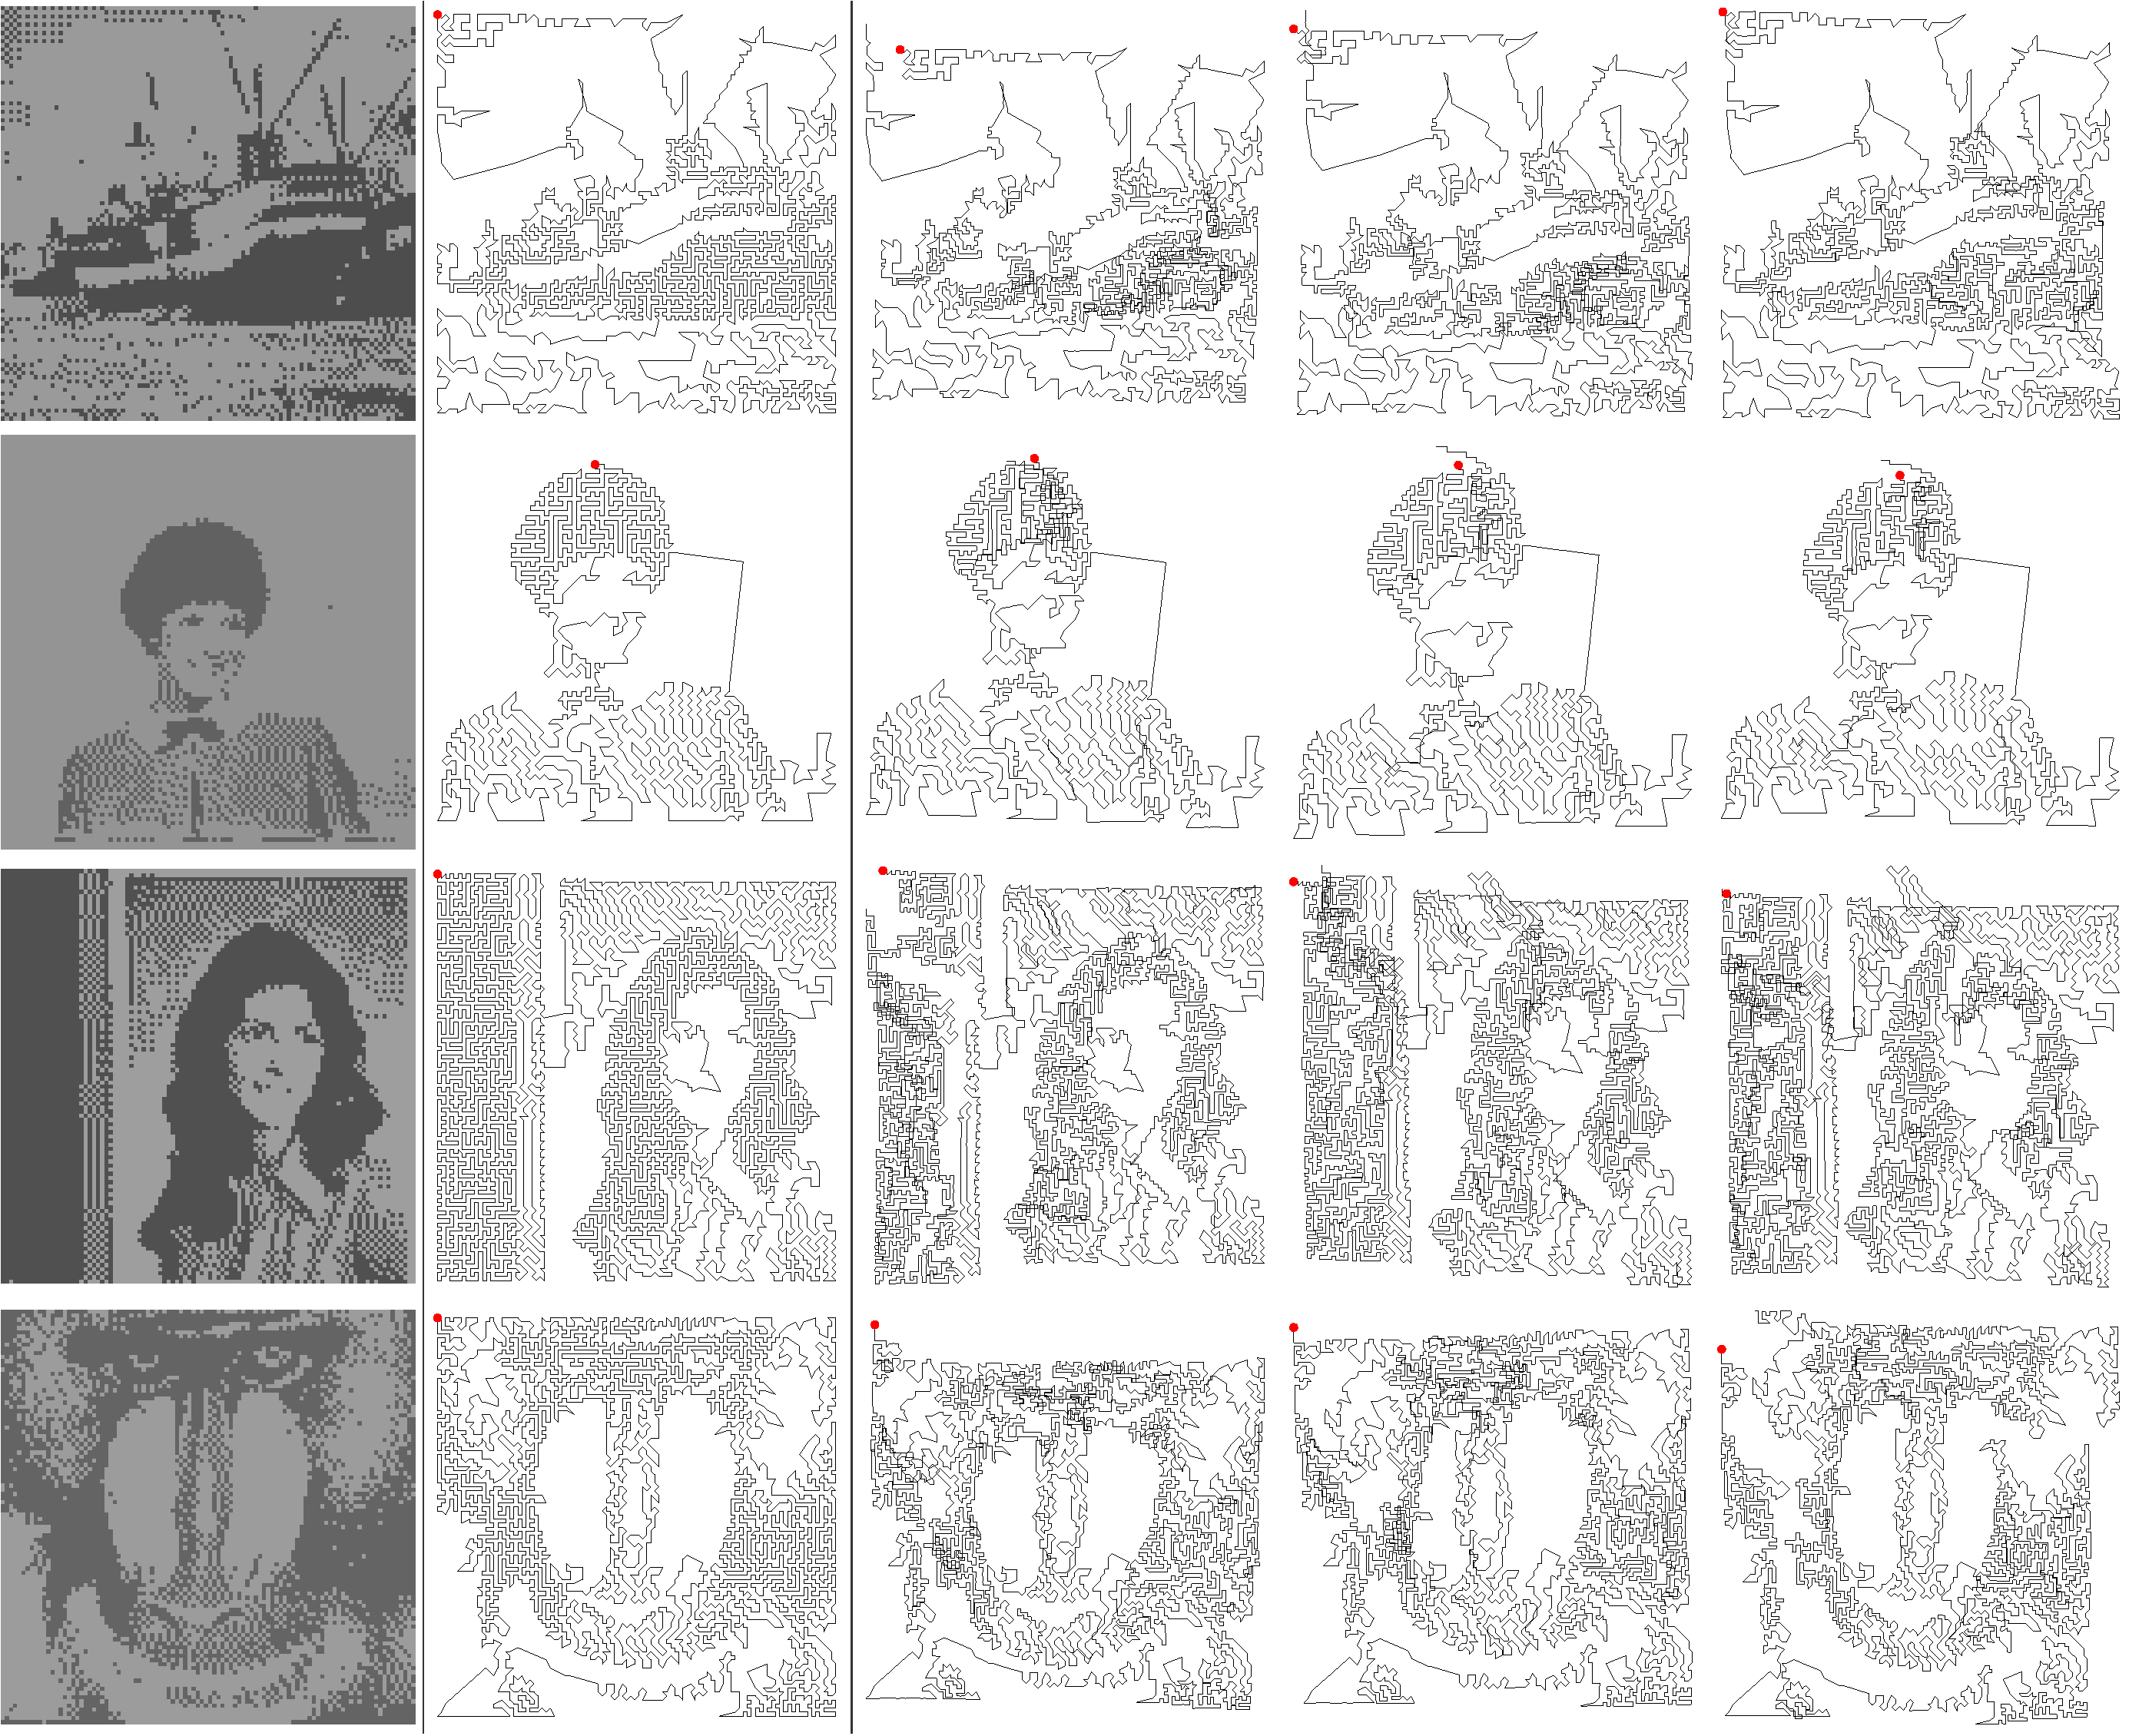
\includegraphics[width=\columnwidth]{Files/gestalt}
            \caption{Samples of noisy paths through some test images. Within each row, the images represent (1) the test image rendered in black and white pixels, (2) the target path corresponding to a tour through the black pixels, and (3--5) samples of noisy attempts at replicating the target path.}
            \label{fig:gestalt}
        \end{figure}

        \begin{figure}[hbt]
            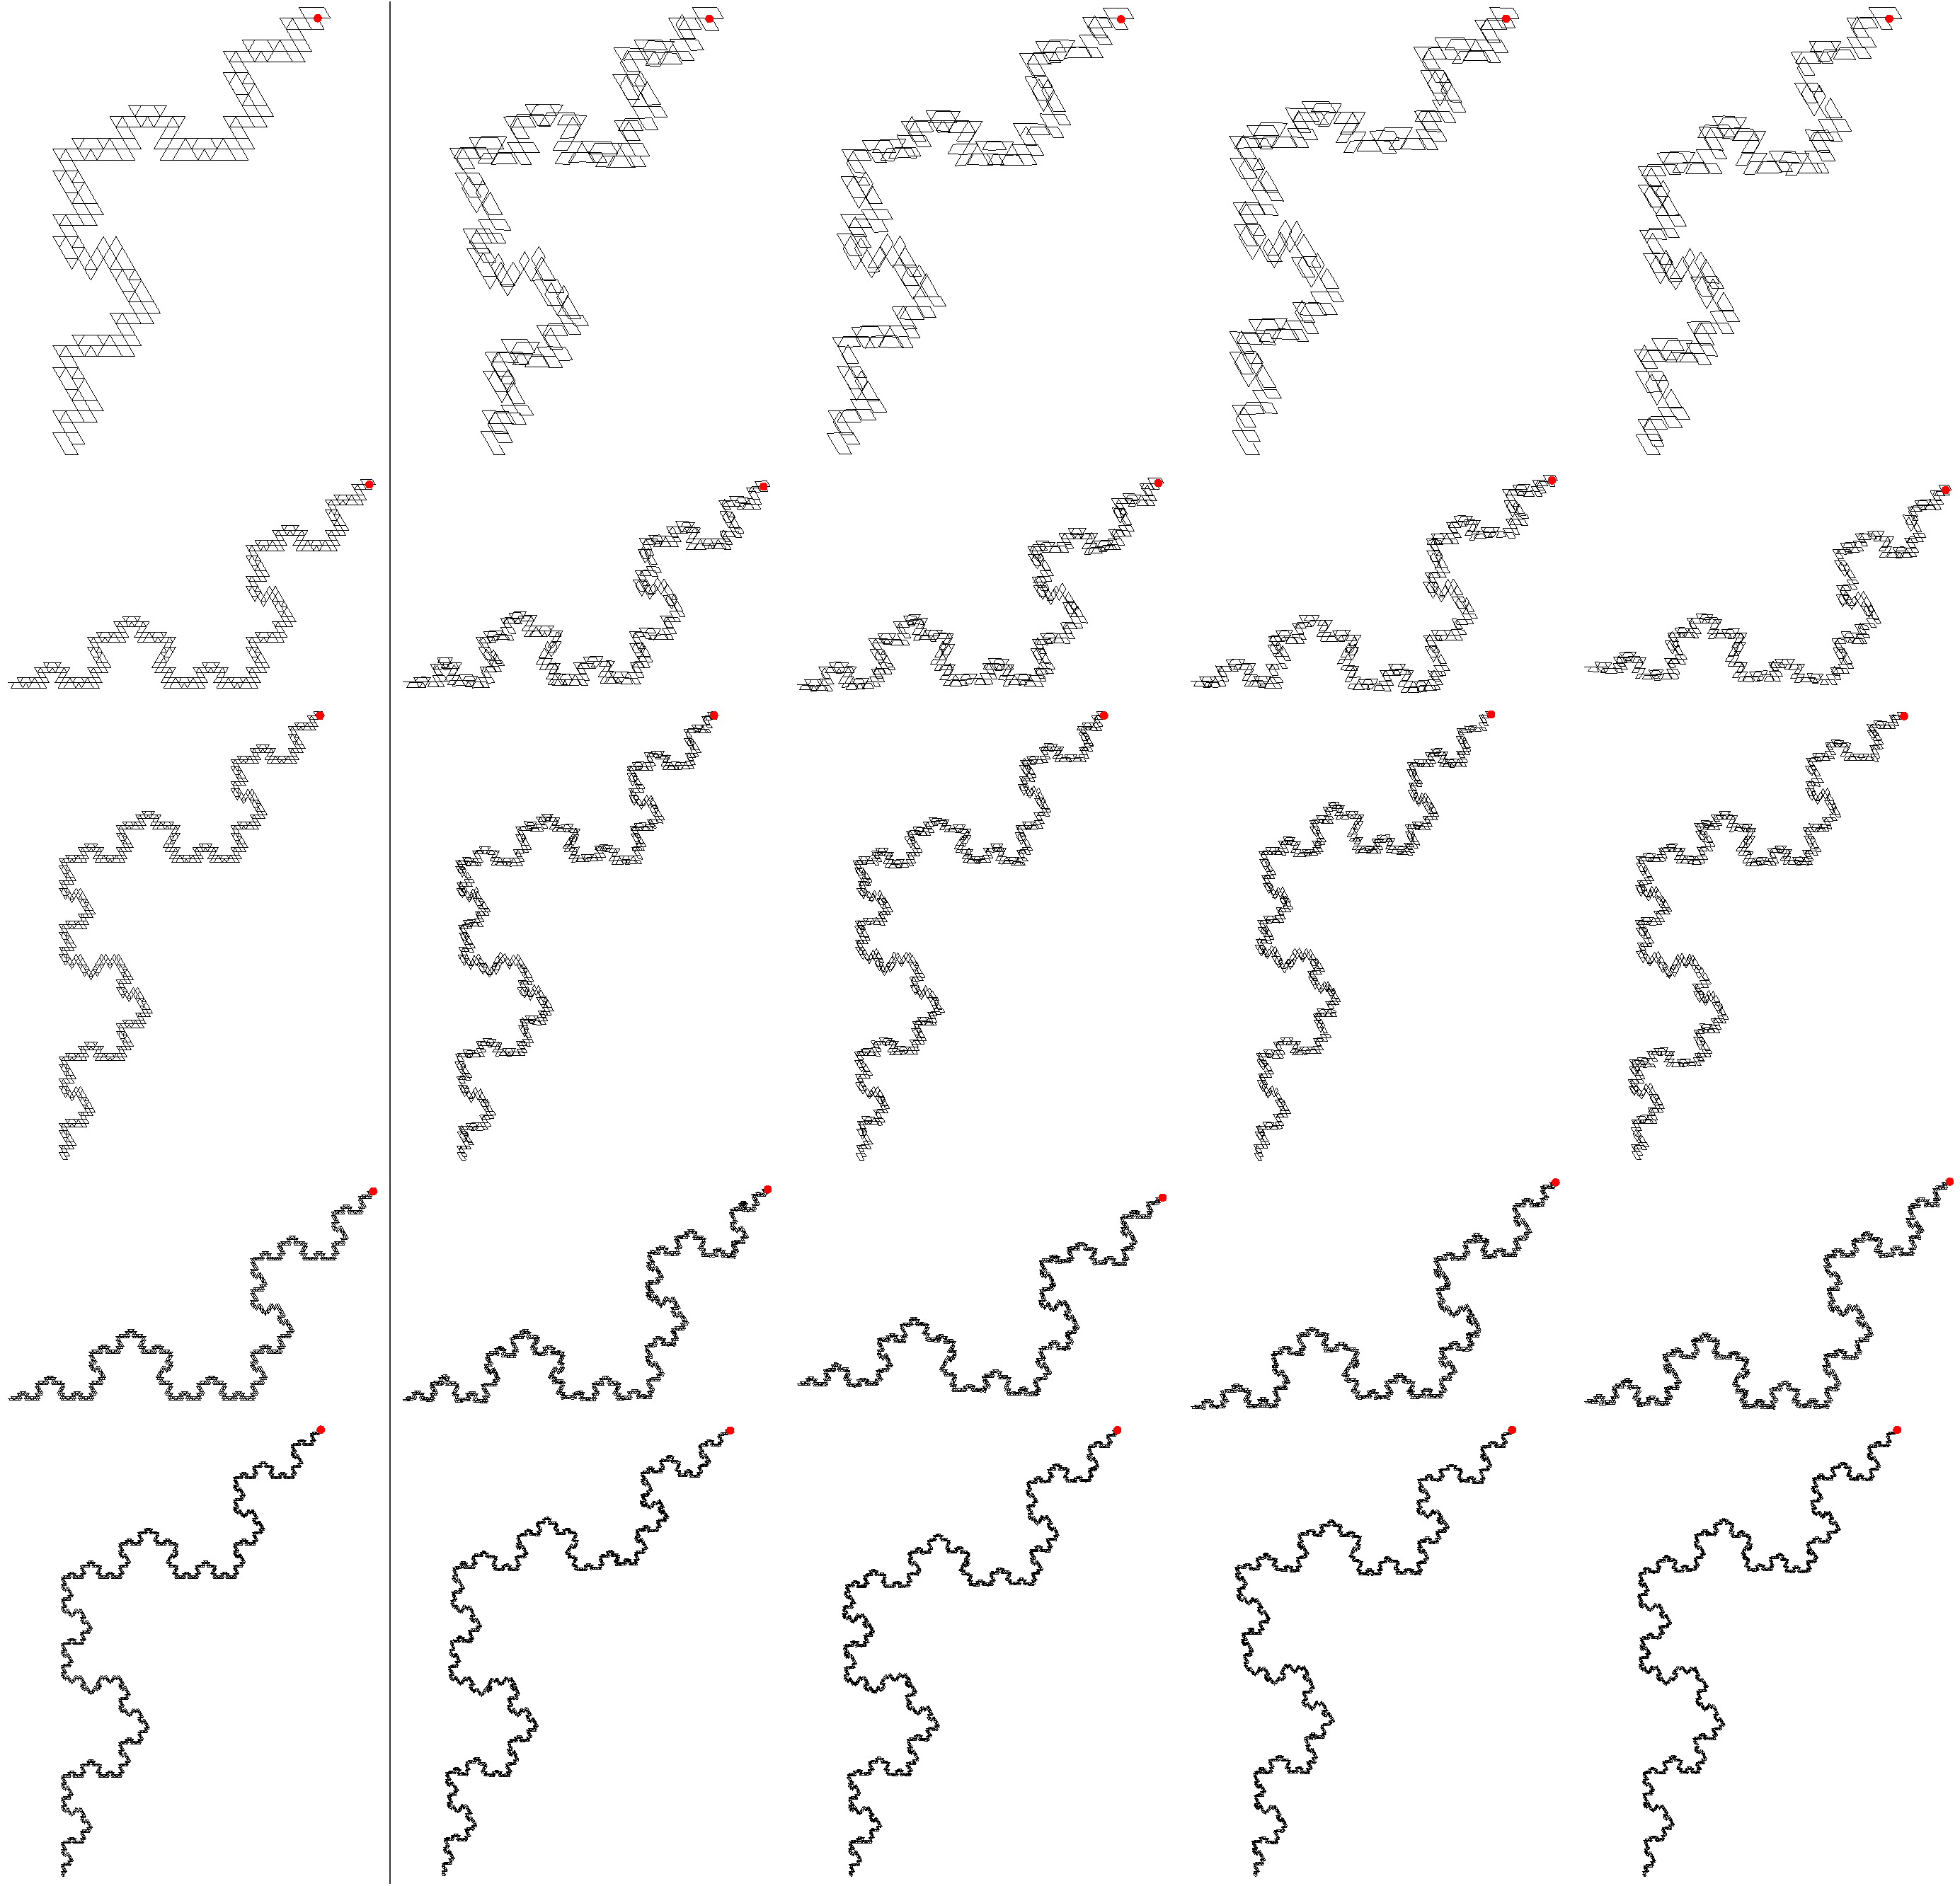
\includegraphics[width=0.5\textheight]{Files/koch}
            \caption{Samples of noisy paths through Koch curves of lengths 1024, 2048, 4096, 8192, and 16384. Within each row, the images represent (1) the target path corresponding to the Koch curve of some length, and (2--5) samples of noisy attempts at replicating the target path.}
            \label{fig:koch}
        \end{figure}

        Some results of sampling target paths are shown in Figures~\ref{fig:gestalt} and \ref{fig:koch}.
        Since the planar dimensions of the longest Koch curve in Figure~\ref{fig:koch} are of the same order of magnitude as the paths through the test images, we can compare the behaviour of their noisy samples.
        It can be seen that the attempts at rendering the test images are fraught with errors whereas the attempts at reproducing the Koch curve appear to converge with increasing length.
        In particular, we find that the most striking errors in Figure~\ref{fig:gestalt} are those that relate to the alignment of features such as the eyes in the second through last test images.
        We note that importance of alignment is a generic feature of visual figures.
        The nature of alignment as small scale order therefore renders figurative art difficult to reproduce with this procedure.
        On the other hand, we find that the long noisy samples of the Koch curve retain, at a large length scale, the scale-invariant shape of the curve.
        These results suggest the existence of a family of noise-robust paths in the plane, containing the Koch curve as one exemplary member.

% Please add to .bib:
% @article{honeywell,
%   title={3-Axis Digital Compass IC HMC5883L: Advanced Information},
%   author={Honeywell},
%   url={http://www.adafruit.com/products/1746}
% }


        \subsubsection{Noise-robust control}
        If instead we want the robot to traverse more general paths, we need to employ a control procedure that is robust to noise.

        Naively, we can take absolute positioning data (GPS, direction from compass) at face value, and we can use\footnote{Given initial position and velocity, we can integrate over acceleration to obtain displacement. This is known as dead reckoning.} relative positioning data (linear and angular acceleration) to compute the robot's motion in between these updates.
        In the absence of noise, this procedure exact.
        But in the presence of noise, it steadily diverges from accuracy with the scale of noise.
        Now intuitively, we would like to give to weight to the forms of positioning data that are less noisy since they introduce less error into our procedure.
        If we carefully model the situation as a stochastic dynamical system, we can obtain rigorous estimates for the robot's position.

        \newcommand\ndistr[2]{\mathcal{N}(#1, #2)}
        \newcommand\noise[1]{\epsilon^{(#1)}}

        \begin{figure}[h]
            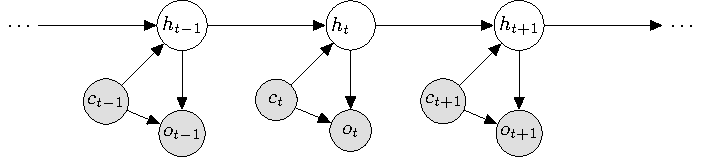
\includegraphics{Files/graphical_model/graphical_model}
            \caption{Causal network of our model, neglecting the noise terms $\noise{h}_t$ (resp. $\noise{o}_t$) that feature independently in each node $h_t$ (resp. $o_t$).
            The graph describes conditional independence between the random variables, such that given $h_t$ and $c_t$ we have that $o_t$ is independent of all $h_\tau, c_\tau, o_\tau$ for all $\tau < t$.}
            \label{fig:SSM}
        \end{figure}

        Following Murphy~\cite{murphy}, consider the state space model whose causal dependence is depicted in Figure~\ref{fig:SSM}.
        At each time step $t = 1, 2, \ldots$, the system is specified by a hidden state $h_t \in \mathbb{R}^{m}$ and an observation $o_t \in \mathbb{R}^{n}$.
        The hidden state corresponds to the underlying state of the robot on the surface of the beach, and the observation corresponds to positioning data retrieved from GPS, compass, and accelerometers.
        If at each time $t$, we send a control signal $c_t$ to the robot, we can write
        \begin{align}
            h_t &= f(h_{t-1}, c_t, \noise{h}_t), \\
            o_t &= g(h_{t}, c_t, \noise{o}_t),
        \end{align}
        where $f$ is a function that models transitions between hidden states, depending on the noise $\noise{h}_t$ associated with the system's evolution; and $g$ is a function that models emissions of observations from hidden states, depending on the noise $\noise{o}_t$ associated with observation.
        For simplicity, we suppose that $f$ and $g$ are both linear in each of their arguments, and that each random variable $h_t, o_t, c_t, \noise{h}_t$, and $\noise{o}_t$ follows a multivariate Gaussian distribution.
        Then we have
        \begin{align}
            h_t &= A_t h_{t-1} + B_t c_t + \noise{h}_t, \\
            o_t &= C_t h_{t} + D_t c_t + \noise{o}_t,
        \end{align}
        where the noise terms\footnote{$\ndistr{\mu}{\Sigma}$ denotes the multivariate Gaussian distribution with vector mean $\mu$ and covariance matrix $\Sigma$.} $\noise{h}_t \sim \ndistr{0}{Q_t}$ and $\noise{o}_t \sim \ndistr{0}{R_t}$ are each centred on zero, and $A_t, B_t, C_t, D_t, Q_t, R_t$ are real matrices of appropriate dimension ($m$ or $n$).
        Formally, this restricts all conditional probability distributions to the class of linear-Gaussian distributions.
        Although we need only that they fall in the exponential family of distributions, the linear-Gaussian case is straightforward to handle analytically.

        If the probability distribution\footnote{The notation $1:t$ denotes, for instance in $o_{1:t}$, the set of observations $o_{1:t} = \{o_1, o_2, \ldots, o_t\}$.} $P(h_t \mid o_{1:t}, c_{1:t}) = \ndistr{\mu_t}{\Sigma_t}$ is Gaussian with mean $\mu_t$ and covariance $\Sigma_t$, it can be shown that the a priori \textbf{prediction} for the state $h_t$, given the observations $o_{1:t-1}$ and control signals $c_{1:t}$, is
        \begin{align}
            &P(h_t | o_{1:t-1}, c_{1:t}) = \ndistr{\mu_{t|t-1}}{\Sigma_{t|t-1}} \\
            \text{where }
            &\begin{cases}
                \mu_{t|t-1} &= A_t \mu_{t-1} + B_t u_t, \\
                \Sigma_{t|t-1} &= A_t \Sigma_{t-1} A_t^\intercal + Q_t.
            \end{cases}
        \end{align}
        Upon observation of $o_t$, we find the optimal \textbf{update} rules
        \begin{align}
            \mu_t &\mapsto \mu_{t|t-1} + K_t r_t, \\
            \Sigma_t &\mapsto (I - K_t C_t) \Sigma_{t|t-1},
        \end{align}
        where the \emph{innovation}
        \begin{align}
            r_t &= o_t - \hat{o}_t \\
            \text{where }\hat{o}_t &= (C_t \mu_{t|t-1} + D_t c_t)
        \end{align}
        is associated with the covariance
        \begin{equation}
            S_t = C_t \Sigma_{t|t-1} C_t^\intercal + R_t
        \end{equation}
        which features in the \emph{Kalman gain matrix}
        \begin{equation}
            K_t = \Sigma_{t|t-1} C_t^\intercal S_t^{-1}.
        \end{equation}
        These rules are optimal in that they minimise the mean-squared error $\langle \lvert o_t - \hat{o}_t \rvert^2 \rangle$.

        By alternating between the \emph{predict} and \emph{update} steps, we recover the Kalman filter algorithm for state estimation.
        Explicitly, these results allow us to compute the exactly optimal prediction for the distribution $P(h_t | o_{1:t}, c_{1:t})$ of the system's state at each point in time, as long as we have access to the
        \begin{enumerate}
            \item dynamical relations $A_t, B_t, C_t, D_t$ of the system,
            \item covariances $Q_t, R_t$ of noise associated with evolution and observation, and
            \item distribution $\ndistr{\mu_0}{\Sigma_0}$ of the initial state $h_0$.
        \end{enumerate}
        In particular, the distribution $P(h_t | o_{1:t}, c_{1:t})$ provides the expected state of the robot on the beach, in addition to the uncertainty in each of the state's parameters.

        If we parametrise the variables in our model such that
        \begin{itemize}
            \item the robot's state $h_t$ is specified by its position, velocity, and orientation;
            \item its observation $o_t$ is specified by its position, velocity, acceleration, and orientation; and
            \item our control signal $c_t$ is specified by predetermined electrical pulses that modulate the speed of the robot's wheels;
        \end{itemize}
        then each of these requirements features in our application of the Kalman filter as follows.
        \begin{enumerate}
            \item The relationship between the robot's position, velocity, acceleration, and motion of its wheels is determined in closed form by Newton's laws.
            \item The covariances in noise can be estimated by fitting repeated measurements to a multivariate Gaussian distribution.
            \item It is common to use a large covariance $\Sigma_0$ for the initial state since it quickly converges to an appropriate value after a few time steps.
                Then the choice of the initial state's mean $\mu_0$ is not significant.\cite{murphy}
        \end{enumerate}

        Some issues that may arise from this approach include its computational cost and the linear-Gaussian model's poor representation of our problem.
        At each time step, the dominant computational costs lie in computing matrix inversion in the Kalman gain matrix $K_t$ and matrix multiplication in the updated covariance matrix $\Sigma_t$, with time complexity $O(n^3)$ and $O(m^2)$ respectively.\footnote{Recall that $m$ is the dimension of the hidden state space and $n$ is the dimension of the observation space.}
        In terms of real time, these scale inversely with the interval $\delta t$ between successive time steps, so that they can easily outpace an embedded system's processor.
        The state space model used above may fail on either of two fronts: linearity and complexity of distribution.
        Since the Gaussian distribution is the maximally entropic probability distribution given the first two moments (mean and variance), divergence from the Gaussian distribution must lie at higher moments.
        Likewise, divergence from linearity must lie at higher orders of the Taylor expansion of $h_t = f(h_{t-1}, c_t, \noise{h}_t)$ and $o_t = g(h_{t}, c_t, \noise{o}_t)$.\footnote{Since these equations describe classical dynamics, we can assume that their Taylor expansions exist.}
        Both of these problems can be addressed by modifying the abstract treatment above---obtaining for instance the extended or unscented variants of the Kalman Filter.


        \mySubsection{Power}{\SSB}\label{outline: power}
            The \gls{Arduino} requires a supply voltage of \SIrange{7}{12}{\volt}. The motors will also require a power supply of \SIrange{5}{12}{\volt}. There are many different types of battery, several of which are appropriate for the robot:

            \paragraph{Single-use alkaline} batteries are common-place and cheap. They come in a variety of sizes and capacities. These batteries must be disposed of after use and can only source small currents (typically no more than 1A). \SI{9}{\volt} PP3 batteries are particularly popular for electronics projects due to their regular shape and convenient connections.
            \paragraph{Rechargeable alkaline or nickel-based} batteries can be re-used. They are often more efficient than their single-use counterparts.
            \paragraph{Lithium Polymer} batteries are often used for remote-controlled vehicles. They have a very high energy-density and can source high currents (>\SI{10}{\ampere}). This makes them particularly suited to powering small vehicles. These batteries are also rechargeable and have short charging times.

            \paragraph{}In order to allow the motors to sink high currents without affecting the supply voltage to the micro-controller, separate power supplies are used for each system: the \gls{Genuino}, the GPS shield and the \gls{magnetometer} (the control system); and the motors and \glspl{servo} (the output system). The lithium polymer batteries are the best choice for the motors since they can source the required currents and are light-weight. The capacity of the battery for the output system is a matter of cost; a high-capacity battery is more convenient but will be more expensive.\\
            The simplest power source for the control system is a \SI{9}{\volt} PP3 battery. The output system is driven by a \SI{7.4}{\volt} \SI{1500}{\milli\ampere\hour} lithium polymer battery\footnote{\pounds{12.00} from Component Shop \textsc{URL:} \url{www.componentshop.co.uk}~~~~\texttt{SKU: LN215}}. This can supply a continuous current of up to \SI{52.5}{\ampere} and can drive both motors at maximum power for 23 minutes. The control and output systems must have a common ground (\SI{0}{\volt}) connection.

    \mySubsection{Motors}{writer TBA}\label{outline: motors}
    \towrite{motors}

\mySection{User interface}{writer TBA}
    \towrite{interface}


\section{Summary and decisions}
    \towrite{summary and decisions}
    \myBlindSubsection{Aims and motivations}{\AH}
    It was agreed by the group that the aim of this project would be the produce a sand art--drawing robot for educational purposes. The intention being that the final product may be utilised to teach pupils, of primary school age, the basic steps involved in coding.
    The children would input a design, using preliminary coding language, into an interface. The children would have to consider the steps involved in producing their desired image and input the details in a manner that a computer can understand. The group's robot would then reproduce this design in the sand.




    \myBlindSubsection{Drawing tool}{writer TBA}


    \myBlindSubsection{Electronics platform and guidance system}{writer TBA}

    Separate power supplies are used for the control system and the motors. The power source for the control system is a \SI{9}{\volt} PP3 battery. The motors are driven by a \SI{7.4}{\volt} \SI{1500}{\milli\ampere\hour} lithium polymer battery.


    \mySubsection{Outline specification}{\textsc{Whole Group}}\label{outline specification}
        \begin{enumerate} %Reference items in this list using \refspec{drawing size} etc.
            \subsubsection{The project}
            \item We shall design and build a prototype robot to draw 2d line drawings in sand.\label{spec: draw}
            \item The robot shall take input from a user which it shall translate into instructions to draw the picture;\label{spec: take input}
            \item the drawings should be ??? \todo{how big will the drawings be?} in size; \label{spec: drawing size}
            \item the robot should be for educational uses. \label{spec: education}

            \subsubsection{Control systems}
            \item The robot shall be controlled with a \gls{Genuino} 101; \label{spec: arduino}
            \item the robot shall use \gls{GPS} for guidance; \label{spec: gps}
            \item the robot should detect objects in front of it. The robot should not collide with objects; \label{spec: detect objects}
            \item the robot should circumvent obstacles.\label{spec: circumvent}

            \subsubsection{The robot hardware}
            \item The robot shall move across the sand using ???\todo{how will it move?}; \label{spec: movement}
            \item the robot shall use ??? \todo{how will it draw?} to draw the images; \label{spec: tool}
            \item the robot shall be built from ??? \todo{what will it be built from?}; \label{spec: material}
            \item the robot shall have dimensions equal to or less than ($56 \times 45 \times 25$) cm. \label{spec: robot size}

            \subsubsection{Safety}
            \item The robot shall have an emergency shut-down switch; \label{spec: kill switch}
            \item the robot should indicate operating faults to the user; \label{spec: error indicator}
            \item the robot should have documentation and instructions for end users. \label{spec: documentation}
        \end{enumerate}
